%
%
%

\documentclass{frontiers}
\usepackage{url}
\usepackage{lineno}
\usepackage[utf8]{inputenc}
\usepackage{listings}

\linenumbers
\renewcommand{\UrlFont}{\ttfamily\small}

%% Configuration of code listings

\definecolor{CodeBackground}{rgb}{0.95, 0.95, 0.9}
\lstset{ %
    language=Python,
    basicstyle=\ttfamily\small,
	backgroundcolor=\color{CodeBackground},
	frame=single,  % the zero-width frame is to make
	framerule=0pt, % the colour extend beyond the listing
	showspaces=false,
	showtabs=false,
	showstringspaces=false,
	extendedchars=\true
}
\lstdefinestyle{display}{
  basicstyle=\ttfamily\footnotesize,
}
%\lstMakeShortInline[basicstyle=\small\ttfamily]{|}

%% Assorted semantic aliases and shortcuts

\newcommand{\latin}[1]{\textit{#1}}
\newcommand{\documentation}{\url{http://neuralensemble.org/neo/}}

%% Commands for use in the editing process. If you wish to add inline comments, please pick a colour and add a new command

\newcommand{\missing}[1]{\textcolor{red}{#1}}
\newcommand{\andrew}[1]{[\textcolor{ForestGreen}{#1}]}
\newcommand{\samuel}[1]{[\textcolor{RubineRed}{#1}]}
\newcommand{\florent}[1]{[\textcolor{Orange}{#1}]}
\newcommand{\robert}[1]{[\textcolor{RoyalBlue}{#1}]}
\newcommand{\thomas}[1]{[\textcolor{Emerald}{TW: #1}]}


% ----------------------------------------------------------------------

\copyrightyear{2013}
\pubyear{}

\def\journal{Neuroinformatics}
\def\DOI{}
\def\articleType{Research Article}
\def\keyFont{\fontsize{8}{11}\helveticabold }
\def\firstAuthorLast{Garcia {et~al.}}
\def\Authors{Samuel Garcia\,$^{1}$, Cyril Dejean\,$^{2}$, Luc Estebanez\,$^{3}$, Domenico Guarino\,$^{3}$, Florent Jaillet\,$^{4}$, Todd Jennings\,$^{5}$, Yann Mahnoun\,$^{6}$, Robert Pröpper\,$^{7}$, Philipp Rautenberg\,$^{8}$, Chris Rodgers\,$^{9}$, Andrey Sobolev\,$^{8}$, Thomas Wachtler\,$^{8}$, Pierre Yger\,$^{3}$ and Andrew P. Davison\,$^{3,*}$}

% Frontiers guidelines: "Affiliations should be keyed to the author's name with superscript numbers and be listed as follows: Laboratory, Institute, Department, Organization, City, State abbreviation (USA, Canada, Australia), and Country (without detailed address information such as city zip codes or street names).
% If one of the authors has a change of address, list the new address below the correspondence details using a superscript symbol and use the same symbol to indicate the author in the author list."
\def\Address{$^{1}$Centre de Recherche en Neuroscience de Lyon, CNRS UMR5292--INSERM U1028--Universite Claude Bernard Lyon 1, Lyon, France \\
$^{2}$Centre de Neurosciences Integratives et Cognitives, CNRS UMR 5228--Université Bordeaux I--Université Bordeaux II, Bordeaux, France \\
$^{3}$Unité de Neurosciences, Information et Complexité, CNRS UPR 3293, Gif-sur-Yvette, France \\
$^{4}$Institut de Neurosciences de la Timone UMR 7289, Aix Marseille Université, CNRS, Marseille, France \\
$^{5}$Division of Neurobiology, Department Biology II, Ludwig-Maximilians-Universität, Munich, Germany \\
$^{6}$Laboratoire de Neurosciences Intégratives et Adaptatives, CNRS UMR 6149--Université de Provence, Marseille, France \\
$^{7}$Neural Information Processing Group, TU Berlin, Germany \\
$^{8}$G-Node, Ludwig-Maximilians-Universität, Munich, Germany \\
$^{9}$University of California, Berkeley, CA, USA}

% Frontiers guidelines: "The Corresponding Author should be marked with an asterisk
% Provide the exact contact address (this time including street name and city zip code) and email of the corresponding author"
\def\corrAuthor{Andrew P. Davison}
\def\corrAddress{UNIC, CNRS, Bât. 32/33, 1 avenue de la Terrasse, 91198 Gif-sur-Yvette Cedex, France}
\def\corrEmail{andrew.davison@unic.cnrs-gif.fr}

% ----------------------------------------------------------------------

\begin{document}
\onecolumn
\firstpage{1}

\title[An object model for electrophysiology]{Neo: a universal object model for handling electrophysiology data in multiple formats}
\author[\firstAuthorLast ]{\Authors}
\address{}
\correspondance{}
\editor{}
\topic{Research Topic: Python in Neuroscience II}

\maketitle
\begin{abstract}

\section{}
% Frontiers guidelines: "As a primary goal, the abstract should render the general significance and conceptual advance of the work clearly accessible to a broad readership. References should not be cited in the abstract." "Maximum length 2000 characters".
% Note: The initial version of the abstract contains 1927 characters (including spaces). The spaces must be included in the count of the maximum length of 2000 characters, see http://www.frontiersin.org/Neuroinformatics/authorguidelines#SummaryTable

In neuroscience, electrophysiological signals are acquired, analysed and visualised using a wide variety of software.
To improve interoperability of different tools and to share data between projects, a common representation of the core data is needed.
To build this common representation, we propose a language independent hierarchical data model suitable for the representation of electrophysiological data acquired from electroencephalographic, intracellular or extracellular recordings, or generated from simulations.
We specify the different considerations taken into account when designing this model and describe it in detail.

Furthermore, we present the Neo package, which is an implementation of this model in Python.
Additionally to providing objects to represent electrophysiology data in memory, this package provides a set of input/output (IO) modules for reading/writing the data from/to a variety of commonly used file formats (including Plexon, Spike2, NeuroExplorer, Axon, AlphaOmega, Micromed, Blackrock, Klustakwik, BrainVision, WinWcp, Elan, Elphy, Neuroshare, TDT, ASCII, HDF5, Matlab and raw binary data).
This package is distributed under a modified BSD license and can be freely downloaded from the Neo project website.
The Neo object model and the associated Python package are deliberately limited to representation of data, with no functions for data analysis or visualization, in order to be as lightweight a dependency as possible.
Packages for neurophysiology data analysis and visualization can then build on top of Neo.

To illustrate the use of the Neo package, we also present a set of common usage examples.

Finally we discuss the current state of the Neo project, specifying the various projects and laboratories contributing to, using, or building on Neo.
We also discuss the sustainability of the project, backed by its active community, as well as its limitations and future direction.

\tiny
 \keyFont{ \section{Keywords:} electrophysiology, interoperability, Python, software, file formats\missing{, ...} } % minimum 5, maximum 8 keywords
\end{abstract}


% ----------------------------------------------------------------------
\section{Introduction}

% Frontiers guidelines: "the introduction should be succinct, with no subheadings."

%  * diversity of analyses/acquisition/plotting systems and lack of interoperability
%  * bridge between experimentalists' and modelers' tools
%  * replication of effort for reading/converting data
%  * existing tools, their limitations (or should that go in Discussion?):
%     - neuroshare
%     - biosig
%     - nitime, good support for continuous data, but not for spikes. Also more integrated with analysis tools, not lightweight
%     - neurapy https://github.com/kghose/neurapy
%     - http://pub.ist.ac.at/~schloegl/matlab/eeg/
%     - SignalML
%  * need to have a model object that embraces complexity of data (heterogeneity, etc.)
%  * open source

In systems neuroscience and computational neuroscience, as in many areas of science, a considerable amount of researchers' time is spent in analysing and visualising data, using some kind of software.
Since science aims always to push at the boundaries of knowledge, it is often the case that no single piece of software is sufficient to perform all the analyses or visualisations of interest for a particular study.
The solution is either to extend the software or to transfer data between software tools.
The former requires both programming skills and effort.
If an entirely novel analysis method is needed, this effort is unavoidable, but if, as is often the case, the required functionality is already provided by a different software tool, transferring the data can in principle be much more efficient.
Unfortunately, in neurophysiology there is a very wide variety of software in use, much of it proprietary and developed by recording hardware manufacturers, and with little in the way of common data formats.
In practice, researchers spend a lot of time and effort converting data between different formats, and those with good programming skills are strongly tempted to reimplement functionality that already exists elsewhere rather than go through a tedious conversion process.
A reduction in the amount of effort required for neurophysiology data conversion could greatly enhance the productivity of the field and reduce duplication of effort. 

Three approaches to reducing the effort of data conversion, and thereby increasing the interoperability of data analysis tools, can be envisioned.
The first is to develop a common file format, capable of containing all data generated by all the different software tools in use.
Having such a file format, the number of possible conversion pathways that must be implemented is greatly reduced.
Ideally, hardware manufacturers would support exporting recorded data in this format.
This approach has been tried with some success in the domain of clinical electroencephalography (EEG) \citep[The European Data Format, EDF;][]{Kemp1992, Kemp2003}, and the Program on Standards for Data Sharing of the International Neuroinformatics Coordinating Facility is currently developing a standard file format for electrophysiology data \citep{Teeters2013} based on the HDF5 format.

The second approach is to define a language that can describe the structure of data files in different formats, and then write descriptions of each of the formats of interest using this language.
Conversion between data formats, or reading a data file into software, can then be fully automated.
This approach was taken by \citet{Durka2004}, who developed the SignalML markup language for describing biomedical time series.

The third approach is to define an application programming interface (API) that takes care of the data conversion, and implement this as a library which can be used by software developers to provide uniform access to data, independent of the file format.
An advantage of this compared to the other two approaches mentioned above is that it encourages modularity in software development: the data-conversion library defines certain data structures that can then be used by developers of analysis and visualization tools, which thereby gain greater interoperability.
A previous effort to define an API for electrophysiology data in neuroscience was taken by a consortium of recording hardware manufacturers, which in 2000 began development of the Neuroshare API \citep{neuroshare}.
The Neuroshare API is available as a C library and as a MATLAB (The Mathworks Inc.) extension.
These are only available for the Windows operating system \samuel{This is not completly true some manufacturers provides some linux lib}\thomas{How about: For most formats, libraries are only available ...}, and are distributed as compiled dynamic-link libraries (DLLs), one per manufacturer; the source code is generally not available.
The API is rather low-level, consisting of a number of functions and low-level data structures such as numerical arrays.

We have developed a novel, object-oriented API for representing electrophysiology data in memory and for reading/writing such data from/to multiple file formats.
The Neo (from \emph{N}euroscience \emph{E}lectrophysiology \emph{O}bjects) API is defined as an object model, and is intended to be able to represent any electrophysiology dataset, from \latin{in vitro} patch-clamp recordings through multi-electrode array recordings to EEG.
We have implemented the Neo object model as a cross-platform, open-source Python package, but it should be possible to implement it in any object-oriented programming language.
An object-oriented API is a natural fit for neuroscience data, and in particular makes it easier to encapsulate data and the associated metadata, hence preserving the information about the experimental context that is needed to correctly interpret and analyse the data.

In this article we describe the design considerations which led to the design of the API, we describe the object model and its Python implementation, then give some examples of using the Neo Python package in real-world situations. Finally, we discuss the advantages and disadvantages of the Neo approach with respect to the other approaches to data sharing and software interoperability mentioned above, and outline possible future directions.


% ----------------------------------------------------------------------
\section{Design considerations}

%  * best practice : units and important metadata (sampling_rate, t_start, ..)
%  * heterogeneity of data
%  * asymmetry of data
%  * scope : data objects only (no visulization or analysis methods)
%    This should be phrased not as a limitation, but rather as a design choice, so that analysis methods are not tied to a proprietary data representation
%  * data can be in chunks : we need a Segment object
%  * compatibility with other scientific libraries 
%  * efficiency for arrays

Starting with the basic requirement that the object model should allow the representation and manipulation of any electrophysiology dataset, we elaborated the design according to the following principles. 

\subsection{Scope}

It was decided that the object model should contain only classes for representing data and for reading/writing data from/to files or databases. Further, the behaviour of these objects should allow only basic manipulations: rearranging datasets, extracting sub-sets. In particular, we wished to specifically exclude visualization or analysis methods, even such simple ones as taking the mean. The motivation for this was to keep Neo as minimal as possible. In our experience developing open-source software, small, focused libraries are much more likely to see widespread uptake.

\subsection{Metadata}

We distinguish essential metadata, which is required for the data to have even minimal meaning rather than just be arrays of numbers, desirable metadata, which is necessary to correctly analyse the data, and additional metadata.
Examples of essential metadata are the sampling interval and the physical units of a recording.
Desirable metadata might include identification of the neuron or brain area from which the recording was made, or the filter settings used.
Additional metadata provide information that is specific to a user or software tool, such as which colour to use when plotting the data in a graphical interface.
The object model should make it impossible to create data objects without essential metadata.
For desirable and additional metadata, it should be straightforward to annotate any object. 
Annotations should take the form either of key--value pairs or of semantic triples. 
In our Python implementation, we chose key--value pairs for simplicity, but we are considering adding support for triples in future versions.
For desirable metadata we add the further requirement that the metadata must be preserved when writing to then reading again from a file or database, whatever the format.

\subsection{Structure}

Experimental protocols in neuroscience are hugely diverse, and may be structured in many ways in terms of stimulus presentation, behavioural responses, pharmacological interventions. The object model should allow at least some of this structure to be represented in the relationships between data objects rather than only as metadata. At least two levels of hierarchical organisation are needed (e.g. a recording session consisting of multiple trials), but non-hierarchical cross-links are also needed.
\samuel{Should we discuss the flexibility to have both continuous recording vs chunk recording ?}

\subsection{Interoperability}

Wherever possible, compatibility with other widely used scientific libraries in a given implementation language should be preserved.

\subsection{Efficiency}

Electrophysiology recordings are often very large, either because recording lasts for a long time, hours or days, or because of recording from many channels. This means that both the object model and its implementation must provide memory- and computation-efficient representations.


% ----------------------------------------------------------------------
\section{Object model}

%  * 3 types : data objects/container objects/grouping objects
%  * 3 types of attributes : required, recommended, and additional
%  * scalar vs non scalar (very briefly)
%  * enumeration of objects
%  * relationships (one to many, many to many)

The Neo object model (version 0.3) consists of \missing{N} classes, which may be divided into three types: data objects, container objects and grouping objects.
Data objects contain numerical data together with associated metadata.
The data types that are represented are 
(i) sampled continuous, analog signals; 
(ii) action potentials (``spikes''), characterized by their time of occurrence and, optionally, their waveforms; 
(iii) events, each of which consists of a time of occurrence and a textual label; and 
(iv) epochs, each of which consists of a start and end time together with a label.
For each data type, the object model provides both a scalar representation (a single instance of a data item, for example, \lstinline`AnalogSignal` and \lstinline`Spike`) and an array representation (e.g., \lstinline`AnalogSignalArray` and \lstinline`SpikeTrain`) in order to provide a choice between flexibility and efficiency in data analysis \andrew{can we provide a more convincing/detailed reason?} \samuel{Unfortunatly no, the real reason was a sad backward compatibility}.
The full list of data objects is as follows:

\begin{itemize}
\item \lstinline`AnalogSignal`: a sampling\thomas{How about ``record'' instead of ``sampling''?} of a continuous, analog signal with a fixed sampling interval.
\item \lstinline`IrregularlySampledSignal`: a sampling of a continuous analog signal with a varying sampling interval.
\item \lstinline`AnalogSignalArray`: a sampling of a multichannel continuous analog signal with a fixed sampling interval.
\item \lstinline`Spike`: one action potential characterized by its time and waveform.
\item \lstinline`SpikeTrain`: a set of action potentials (spikes) emitted by the same unit in a period of time (with optional waveforms).
\item \lstinline`Event` and \lstinline`EventArray`: a time point representing an event in the data, or an array of such time points.
\item \lstinline`Epoch` and \lstinline`EpochArray`: an interval of time representing a period of time in the data, or an array of such intervals.
\end{itemize}

Container objects provide a simple hierarchical grouping of data. 
A \lstinline`Segment` may contain any of the data object types above provided all the objects share a common time basis, i.e. they all represent data recorded at the same time without breaks in the recording\thomas{``without breaks ...'' might be misunderstood. Remove?}. 
A \lstinline`Block` is the top-level container, and contains \lstinline`Segment`s and \lstinline`RecordingChannelGroup`s (see below).
To illustrate this further, in the common experimental paradigm of running multiple trials, i.e., presenting the same stimulus multiple times, the data from each trial would be stored in a \lstinline`Segment`, and all the \lstinline`Segment`s stored in a single \lstinline`Block`. 

Grouping objects express the relationships between data objects, such as which signals were recorded on which electrodes, which spike trains were obtained from which membrane potential signals, etc.
They contain references to data objects that cut across the simple container hierarchy.
The grouping objects are as follows:

\begin{itemize}
\item \lstinline`RecordingChannel`: links \lstinline`AnalogSignal` \samuel{\lstinline`SpikeTrain` are not linked by RC and and I just see that figure 1 is wrong on that} objects that come from the same logical and/or physical channel inside a \lstinline`Block`, possibly across several \lstinline`Segment` objects.
\item \lstinline`RecordingChannelGroup`: a group for associated \lstinline`RecordingChannel` objects. This has several possible uses: 
(i) for linking several \lstinline`AnalogSignalArray` objects across several \lstinline`Segment` objects inside a \lstinline`Block`;
(ii) for multielectrode arrays, where spikes may be recorded on more than one recording channel, and so the \lstinline`RecordingChannelGroup` can be used to associate each \lstinline`Unit` with the group of recording channels from which it was calculated;
(iii) for grouping several \lstinline`RecordingChannel` objects. There are many use cases for this. For instance, for intracellular recording, it is common to record both membrane potentials and currents at the same time, so each \lstinline`RecordingChannelGroup` may correspond to the particular property that is being recorded. For multielectrode arrays, \lstinline`RecordingChannelGroup` is used to gather all \lstinline`RecordingChannel` objects of the same array.
\item \lstinline`Unit`: a \lstinline`Unit` gathers all the \lstinline`SpikeTrain` objects within a common \lstinline`Block`, possibly across several \lstinline`Segments`, that have been emitted by the same cell. A \lstinline`Unit` is linked to \lstinline`RecordingChannelGroup` objects from which it was detected.
\end{itemize}

Another way to think of this is that container objects providing a grouping across time while grouping objects provide a grouping across space.
Figure~\ref{fig:overview} provides an overview of the Neo objects and their relationships.


\begin{figure}
\centering
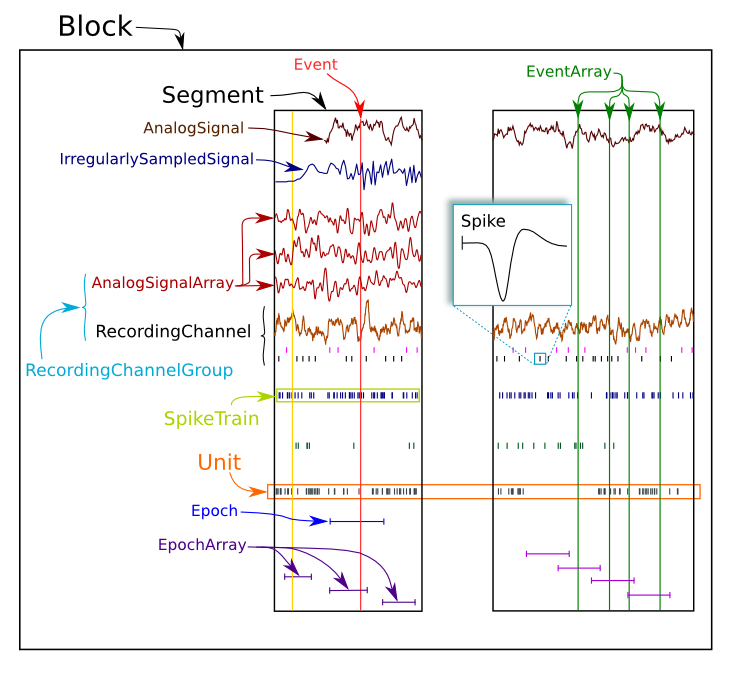
\includegraphics[width=0.8\textwidth]{figures/base_schematic2_lowres}
\caption{An illustration of the data types supported by Neo and their grouping into containers.}\label{fig:overview} 
\end{figure}
% Note: Figures should not be included in the final submitted LaTeX file, but uploaded separately when submitting the article. Frontiers will add the figures at the end of the provisional pdf.
%
% Figure requirements:
%
%  Image Type       Format      Color Mode   Resolution
%  Line Art    TIFF, EPS, JPEG     RGB      900 - 1200 dpi
%  Halftone    TIFF, EPS, JPEG     RGB      300 dpi
%  Combination TIFF, EPS, JPEG     RGB      600 - 900 dpi
%
% * The smallest visible text is no less than 8 points in height, when viewed at actual size.
% * Solid lines are not broken up.
% * Image areas are not pixelated or stair stepped.
% * Text is legible and of high quality.
% * Any lines in the graphic are no smaller than 2 points width.


\subsection{Object attributes}

Most objects, and in particular all of the data objects, have a number of \emph{required} attributes.
These are essential metadata without which the numerical data values contained in the object cannot be interpreted.
For example, in the case of \lstinline`AnalogSignal`, the required attributes are the sampling interval (or, equivalently, the sampling rate) and the units of the signal, for example ``millivolts'' in the case of the membrane potential. \samuel{you do not mention 'tstart' (also required) intentionally ?} 
All attributes that represent physical quantities must state the units, for example, the sampling rate could be given as ``10 kHz''.

In addition to the required attributes, each object has a number of \emph{suggested} attributes.
These attributes are intended to contain metadata that are not essential for working with the objects, but that are likely to be useful in developing analysis methods, automatic graph generation, tracking provenance, etc.
Examples of such suggested attributes are \lstinline`name`, \lstinline`rec_datetime` (the date and time of the original recording) and \lstinline`file_origin` (the filesystem path or URL of the original data file from which the data were read).
The number of suggested attributes is likely to increase in future as structured terminologies and ontologies for neurophysiology are developed.
Full details about required and suggested attributes are available in the Neo documentation, online at \documentation.

Finally, any object may contain any number of additional attributes or annotations.
Such annotations may be numerical or text values, arrays of such values, or dictionaries/hash tables containing such values.
They are intended to contain any information that may be useful in subsequent processing of the data, for example metadata describing the experimental protocol.


\subsection{Relationships between objects}

The functions of the container and grouping objects are based on lists of references to other objects.
For example, \lstinline`Block` has an attribute \lstinline`segments`, which is a list of references to all the \lstinline`Segment` objects contained in that \lstinline`Block`.
Such relationships are bi-directional, for example each \lstinline`Segment` has an attribute \lstinline`block` pointing to the \lstinline`Block` within which it is contained.
Figure~\ref{fig:relationships} shows all of these relationships.
More detail is available in the online documentation.

\begin{figure}
\centering
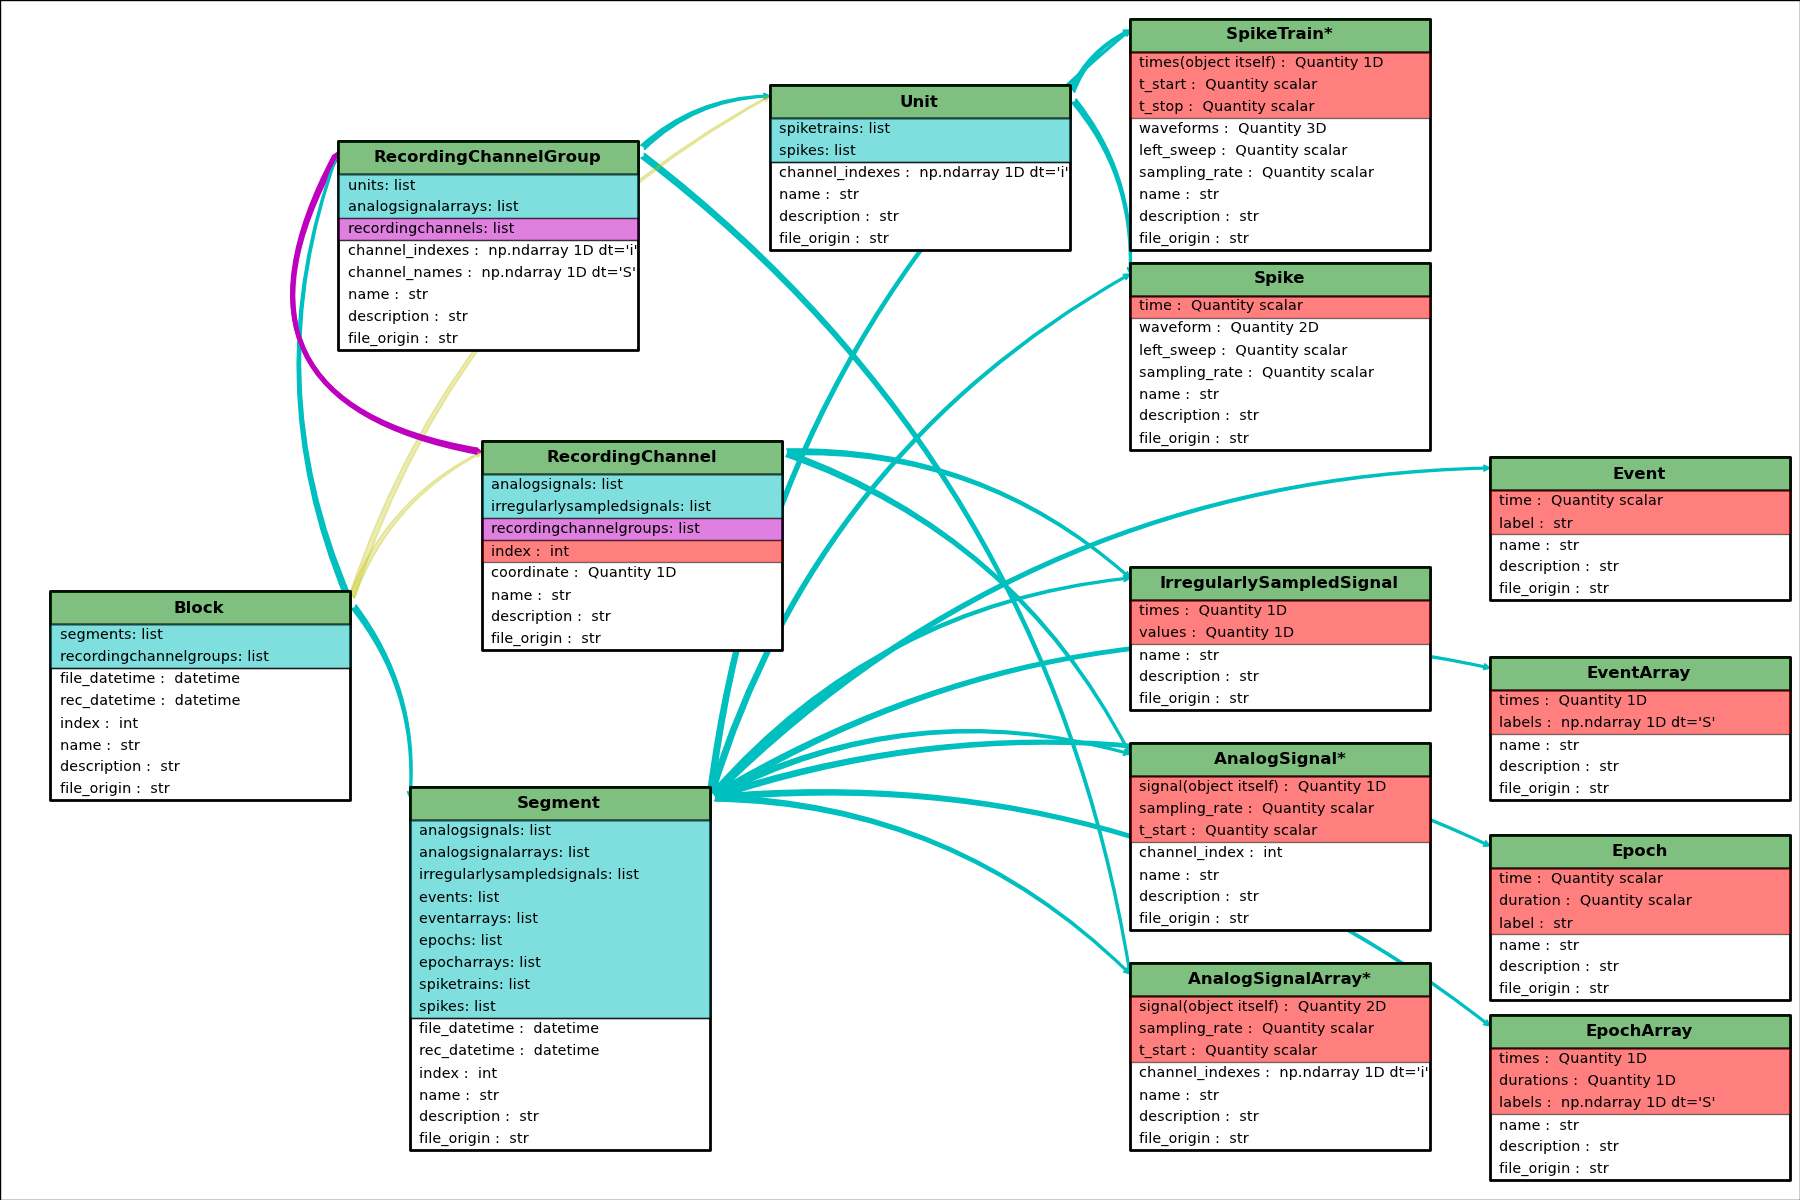
\includegraphics[width=0.8\textwidth]{figures/simple_generated_diagram.png}
\caption{The Neo object model: the principal classes and their relationships. \missing{This is a temporary version of the figure. A better version needs to be created.}}\label{fig:relationships}
\end{figure}

\subsection{Implementation in Python}

%  * numpy and quantities
%  * classes that inherit from quantities : arguments for and against the choice to use inheritance
%  * annotations in dict
%  * initialization (required, recommended, and additional)
%  * relationships - with python list (simple but comes with limits)

When implementing the object model in a specific language, ease-of-use considerations come to the fore.
If a package or library is to gain widespread adoption, it should be easy to build and install on different platforms, and should be interoperable, as much as possible, with existing tools and existing code for handling electrophysiology data in that language.

In the case of Python, the latter consideration dictates that Neo must be based on NumPy \citep{Oliphant2007}, the \latin{de facto} standard for numerical computing in Python.
NumPy provides a powerful, $N$-dimensional array object that can contain integers, floating point numbers, strings or other Python objects.
A given numerical array can have any combination of precision and byte-order.
Most array operations are implemented in C or Fortran for efficiency.
The principal choice in implementing the Neo object model in Python is whether the classes for data objects should inherit from the NumPy \lstinline`ndarray` class (a Neo class \emph{is} a NumPy array) or whether to use composition (where the Neo class has a \lstinline`data` attribute which is a NumPy array).
Inheritance has two important advantages:
(i) existing code that works with NumPy arrays will work with Neo data objects without modification;
(ii) Neo objects gain most of the functionality of NumPy arrays ``for free'', i.e. we do not have to reimplement this functionality. 
A number of operations on, and methods of, NumPy arrays have to be reimplemented or extended for Neo objects, in order to preserve the extra metadata carried by Neo objects, but these would in any case have to be implemented if taking the composition approach.
The principal disadvantage of the inheritance approach is complexity: creation of classes and types is one of the more difficult parts of the Python language.

The second major choice was how to handle units.
Several Python packages are available for handling units and physical quantities in Python.
The decision to use inheritance for NumPy support narrows down the choice.
We chose to use the Quantities package (\url{http://pythonhosted.org/quantities/}), which provides a \lstinline`Quantity` class that inherits from the NumPy \lstinline`ndarray` class and adds a concept of physical dimensions and units.
This means that trying to add a \lstinline`Quantity` array with dimensions of voltage to an array with dimensions of current will produce an exception, while adding an array in millivolts to an array in volts will perform scaling so as to give the correct result.
The particular choice of Quantities is not limiting.
It would be possible to replace it with another units package that subclasses \lstinline`ndarray`, such as Pint (\url{http://pint.readthedocs.org/}), without changing the Neo interface.

In summary, then, the classes for the Neo data objects all inherit from \lstinline`Quantity`, and so gain checks for dimensional consistency for free, in addition to the large amount of functionality inherited from \lstinline`ndarray`.
Neo objects add further checks (for example, trying to add together two \lstinline`AnalogSignal`s with different sampling rates produces an exception) and further operations (for example, it is possible to slice \lstinline`AnalogSignal`s and \lstinline`SpikeTrain`s according to time as well as according to index).

\missing{[We need to explain why we didn't use Pandas, nitime, or any of the other Python packages for working with time series data.]}
Other Python packages for working with time series data do not fill the niche that Neo does. 
The core function of Neo is data representation. 
The pandas package (\url{http://pandas.pydata.org}) is a general toolkit for working with heterogeneous data. 
Neo contains functionality specific for neural data analysis, such as grouping of channels by anatomical location.
Another package, nitime (\url{http://nipy.org/nitime}), provides algorithms for time-series analysis that are tailored toward neuroscience data.
In contrast, Neo intentionally does not provide algorithms for data analysis since this will vary widely across users.
Overall, Neo provides functionality that is specific to neuroscience data (unlike Pandas) but not specific to particular applications within neuroscience (unlike nitime).
This means that Neo is ideally situated to be a common format for neuroscientists, who may then analyze the data using the tools provided by other packages as desired.

\missing{[Should perhaps say more about the various methods available on AnalogSignals, etc.?]}
Because the primary function of Neo is neural data representation, the methods provided fall into two categories: 1) reading from the various formats used by hardware manufacturers; 2) linking the resulting objects in a neuroscientifically meaningful way.
The first type of linkage is spatial: AnalogSignal object may be added to RecordingChannel objects, and RecordingChannel objects added to anatomically defined RecordingChannelGroup objects.
The second type of linkage is temporal: AnalogSignal objects also belong to a Segment object (representing a period of time), and Segment belongs to Block (representing an entire experiment).
Typically the provided IO methods construct the linkages in this hierarchy automatically.
Then the user may iterate over the data in whatever way is most intuitive for the application: either temporally (trial by trial within a session) or spatially (channel by channel within the brain).

\missing{[Discuss the implementation of relationships]}
\samuel{ isn't redoundant with  'subsection Relationships between objects' ? }

\missing{[Discuss the implementation of annotations]}

The Neo package is available from the Python Package Index (\url{https://pypi.python.org/pypi/neo/} and as a Debian package through NeuroDebian \citep{Halchenko2012}.
The core of Neo works with both Python 2 (version 2.6 or later) and Python 3 (version 3.2 or later).
For some file formats, only Python 2 is currently supported.
Full documentation is available online at \documentation.
There is an extensive test suite, and the project makes use of continuous integration (\url{https://travis-ci.org/NeuralEnsemble/python-neo}) to rapidly catch regressions.


% ----------------------------------------------------------------------
\section{Reading and writing data with multiple file formats}

%  * API flexible because heterogenous data format
%  * one class = one format
%  * mode explenation :  file/dir/database (different karg in __init__)
%  * Supported objects/readable objects  (monolitic read vs partial reading)
%  * Lazy reading concept (include Robert's proposal for post reading lazy object)
%  * cascade reading concept
%  * use memmap when possible
%  * explanation for proprietary formats : reverse engineering + version formats problem

In addition to implementing the Neo object model as a Python API, the Neo Python package also provides a set of input/output (IO) modules for various neurophysiology file formats, including proprietary formats (e.g. Plexon, Spike2, NeuroExplorer, Axon, AlphaOmega, Micromed and Tucker-Davis), the formats used by various open-source tools (e.g. Klustakwik, Elan \florent{Elan does not seem to be open-source, it seems to be only freeware. From the website http://elan.lyon.inserm.fr you can download all kinds of binaries, but no source.}, WinEdr) and generic file formats such as Matlab, ASCII and HDF5. 
In most cases, the proprietary formats are read-only, while the more open and generic formats support both reading and writing.

The inclusion of this functionality in the Neo package has several benefits:
(i) it demonstrates the universality of the object model, which is able to represent the data from all of these different file formats;
(ii) it is an important part of realising our goal of improving interoperability of different tools and the ease of sharing data between different projects;
(iii) it provides an immediate benefit to users, thus driving uptake of the Neo software;
(iv) tool developers can use Neo as a basis and immediately gain the benefit of supporting multiple file formats, without them having to implement such support themselves.


For each file format there is a separate Python class, each of which implements the same interface. Reading data for a given format can be as simple as:

\begin{lstlisting}[style=display]
from neo.io import MyFormatIO
reader = MyFormatIO(filename="myfile.dat")
data = reader.read()
\end{lstlisting}

However, given the large size of many neurophysiology datasets, it is not always desirable to load all the data into memory at once. The full interface therefore offers more fine-grained control.
All read functions have two optional parameters: \lstinline`cascading` and \lstinline`lazy`.
When \lstinline`cascading` is set to false, only a single object is loaded and none of its references to other objects are populated.
The \lstinline`lazy` parameter does not influence if linked objects are loaded, but determines the treatment of data objects: When \lstinline`lazy` is true, the numerical data is not loaded but data objects are still created, including all of their properties. This allows examining the contents of files with a substantially smaller memory footprint. IO classes can implement a method to load the full version of a lazily loaded object once the numerical data is required.

The neo.io API also takes into account that a dataset does not necessarily come from a single file. Some software can provide recordings in a directory or in a database. Such cases are taken into account through the attribute \lstinline`mode` in each IO class. The behaviour is changed only at the instantiation:

\begin{lstlisting}[style=display]
from neo.io import MyFormat1IO, MyFormat2IO
reader1 = MyFormat1IO(filename="myfile.dat")  # MyFormat1IO.mode = 'file'
reader2 = MyFormat2IO(dirname="/path_to_dataset")   # MyFormat2IOmode = 'dir'
\end{lstlisting}

Some file formats internally store arrays in a compact continuous way. In such cases, classes implementation use the numpy.memmap mechanism. It reduces the memory footprint and allows to access transparently files that do not fit into the entire memory. \robert{I believe that this is not working because of quantities (the data is always fully read). Do we have proof that it actually works?} \samuel{Are you sur that quantity do a copy each time ? if yes we need to remove this memmap discussion}
For the implementation of file readers, an early difficulty was collecting information about specification for proprietary file formats. This tedious task was accomplished with several methods (i) asking manufacturers to open these specifications, (ii) reading code from other packages (iii) reading C header files (iiii) basic reverse engineering with hexadecimal editors. Nowadays, many manufacturers provide their file specifications in the user documentation.
The main difficulty remains in the versioning of these specifications. In general, the internal file formats do not change much over time, but sometimes some problematic changes occur, making the classes non backward compatible. This has been taken in account for some file formats. The \lstinline`AxonIO` implementation is a good example where two very different versions of the same file format can be read transparently. Unfortunately, this is not the case for all classes and the effort must continue.

\samuel{[other things to mention: (4) the idea of Neo as a place to collect and harmonize different Python scripts for different formats from all over the web = better in discussion no?]}


\missing{[should perhaps go into more detail on Matlab and HDF5 formats]}
Two of the IO classes do not implement an already existing format : NeoHdf5IO and NeoMatlabIO. Both have in common to use a generic file format, respectively hdf5 and matlab that allows internal organisation of the data in a tree. So in that classes the Neo hierarchical model is directly used to store objects in the file. In short the organisation in the file is close to the Neo objects organisation. In that way, two new file formats are proposed. They are efficient because built on mature library (hdf5 and matlab) and quite universal. And furthermore, their implementation are generic because they are based on the object model descriptions.



% ----------------------------------------------------------------------
\section{Usage examples}

\missing{Reuse use cases from online docs, unless someone has some nicer examples to contribute?}

%  * Recording multiple trials from multiple channels = acces by Segment or acces by Channel
%  * Recording spikes from multiple tetrodes

\subsection{Recording multiple trials from multiple channels}


In this example we suppose that we have recorded from an 8-channel probe, and that we have recorded three trials/episodes. We therefore have a total of 8 x 3 = 24 signals, each represented by an AnalogSignal object.

On Figure~\ref{fig:usecase1}, our entire dataset is contained in a Block, which in turn contains:
\begin{itemize}
\item 3 Segment objects, each representing data from a single trial,
\item 1 RecordingChannelGroup, composed of 8 RecordingChannel objects.
\end{itemize}

\begin{figure}
\centering
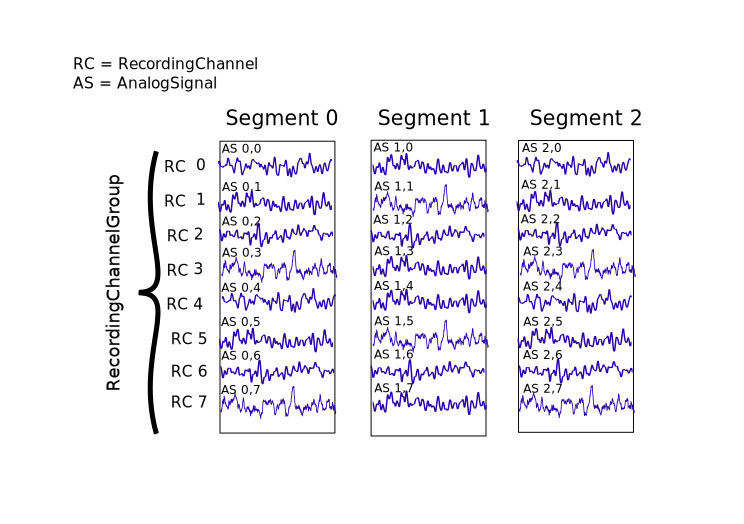
\includegraphics[width=0.8\textwidth]{figures/usecase1}
\caption{An illustration of recording multiple trials from multiple channels.}\label{fig:usecase1} 
\end{figure}

\subsubsection{Temporal (by segment)}

In this case you want to go through your data in order, perhaps because you want to correlate the neural response with the stimulus that was delivered in each segment. In this example, we’re averaging over the channels:

\begin{lstlisting}[style=display]
import numpy as np
from matplotlib import pyplot as plt

for seg in block.segments:
    print("Analyzing segment %d" % seg.index)

    siglist = seg.analogsignals
    avg = np.mean(siglist, axis=0)

    plt.figure()
    plt.plot(avg)
    plt.title("Peak response in segment %d: %f" % (seg.index, avg.max()))
\end{lstlisting}

\subsubsection{Spatial (by channel)}

In this case you want to go through your data by channel location and average over time. Perhaps you want to see which physical location produces the strongest response, and every stimulus was the same:

\begin{lstlisting}[style=display]
# We assume that our block has only 1 RecordingChannelGroup
rcg = block.recordingchannelgroups[0]:
for rc in rcg.recordingchannels:
    print("Analyzing channel %d: %s", (rc.index, rc.name))

    siglist = rc.analogsignals
    avg = np.mean(siglist, axis=0)

    plt.figure()
    plt.plot(avg)
    plt.title("Average response on channel %d: %s' % (rc.index, rc.name)
\end{lstlisting}


\subsection{Recording spikes from multiple tetrodes}

Here is a similar example in which we have recorded with two tetrodes and extracted spikes from the extra-cellular signals. The spike times are contained in SpikeTrain objects.

On Figure~\ref{fig:usecase2}, again, our data set is contained in a Block, which contains:

\begin{itemize}
\item 3 Segments (one per trial).
\item 2 RecordingChannelGroups (one per tetrode), which contain:
  \begin{itemize}
  \item 4 RecordingChannels each
  \item 2 Unit objects (= 2 neurons) for the first RecordingChannelGroup
  \item 5 Units for the second RecordingChannelGroup.
  \end{itemize}
\end{itemize}

In total we have 3 x 7 = 21 SpikeTrains in this Block.

\begin{figure}
\centering
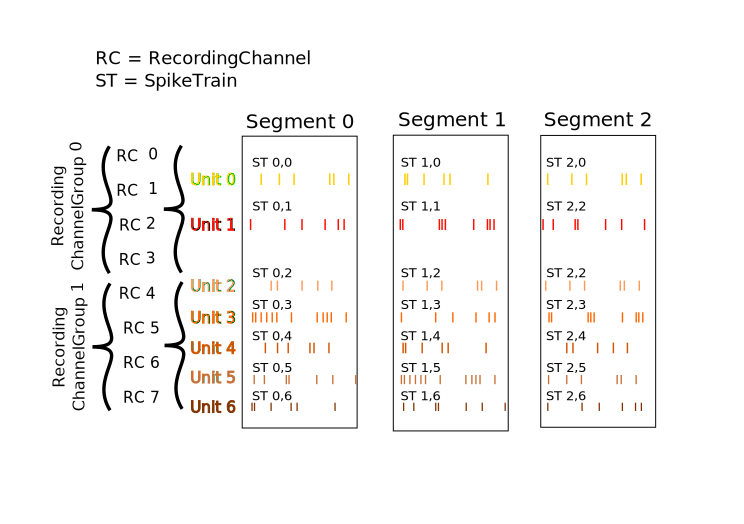
\includegraphics[width=0.8\textwidth]{figures/usecase2}
\caption{An illustration of recording spikes from multiple tetrodes.}\label{fig:usecase2} 
\end{figure}



There are three ways to access the SpikeTrain data:
\begin{itemize}
\item by Segment
\item by RecordingChannel
\item by Unit
\end{itemize}

\subsubsection{By Segment}

In this example, each Segment represents data from one trial, and we want a PSTH for each trial from all units combined:

\begin{lstlisting}[style=display]
for seg in block.segments:
    print("Analyzing segment %d" % seg.index)
    stlist = [st - st.t_start for st in seg.spiketrains]
    plt.figure()
    count, bins = np.histogram(stlist)
    plt.bar(bins[:-1], count, width=bins[1] - bins[0])
    plt.title("PSTH in segment %d" % seg.index)
\end{lstlisting}

\subsubsection{By Unit}

Now we can calculate the PSTH averaged over trials for each unit, using the block.list\_units property:

\begin{lstlisting}[style=display]
for unit in block.list_units:
    stlist = [st - st.t_start for st in unit.spiketrains]
    plt.figure()
    count, bins = np.histogram(stlist)
    plt.bar(bins[:-1], count, width=bins[1] - bins[0])
    plt.title("PSTH of unit %s" % unit.name)
\end{lstlisting}


\subsubsection{By RecordingChannelGroup}
Here we calculate a PSTH averaged over trials by channel location, blending all units:
\begin{lstlisting}[style=display]
for rcg in block.recordingchannelgroups:
    stlist = []
    for unit in rcg.units:
        stlist.extend([st - st.t_start for st in unit.spiketrains])
    plt.figure()
    count, bins = np.histogram(stlist)
    plt.bar(bins[:-1], count, width=bins[1] - bins[0])
    plt.title("PSTH blend of tetrode  %s" % rcg.name)
\end{lstlisting}



% ----------------------------------------------------------------------
\section{Discussion}

% Frontiers guidelines: "This section may be divided by subheadings. Discussions should cover the key findings of the study: discuss any prior art related to the subject so to place the novelty of the discovery in the appropriate context; discuss the potential short-comings and limitations on their interpretations; discuss their integration into the current understanding of the problem and how this advances the current views; speculate on the future direction of the research and freely postulate theories that could be tested in the future."

%\missing{[Recap what we have shown in this paper]}:
We have presented the Neo object model and its implementation in Python.
We have shown how this model and the corresponding Python package are designed to allow for convenient and efficient representation of all kinds of electrophysiological data, from spikes to broadband continuous signals, with support for all the common recording technologies, including multi-channel systems like tetrodes.
Furthermore, we have illustrated the practical use of the Neo Python package through examples in typical real-world situations.

The universality of the Neo object model for the representation of electrophysiolgical data coupled with the availability of a large set of IO modules for common file formats in the Python package makes Neo a very convenient base package to build on when developing software to manipulate, analyse or display electrophysiological data in Python.

It thus fulfils our initial goal as a tool to facilitate data sharing and conversion, as well as software interoperability, with the hope that Neo will become the standard base package for the community of Python developers working with electrophysiological data.

\missing{[Discuss how Neo relates to previous/future standardization efforts (e.g. Neuroshare, EDF, Pandora) and to alternative existing tools in the same domain (BioSig, Nitime, pandas, SignalML]}

%Impact : projects using neo
%-----------------------------------------
  
%  * impact (major or null) depends on whether adopted or not
%  * brief intro on sustainability (several lab and several dev)

%Each dev write some lines for their project, then we can eliminate redunduancies between accounts

We were able to demonstrate that NEO facilitates development of various types
of software: entire services providing data management facilities including
electrophysiological data, local tools at the neuroscientific workbench like
simulators, and even individual scripts of scientists analysing their data.

%\missing{... [say more about the significance of this]}
A number of projects and laboratories are using Neo. A total of 5 differents laboratories are developping and  using dailly tools based on neo. A brief overview of theses projects is helpfull to gauge the benefit.


The German INCF Node (G-Node) has adopted the Neo model for the representation of electrophysiological data at its data management platform (portal.g-node.org/data/).
Purpose of the platform is to provide a centralized system for organizing and sharing of electrophysiology data.
A major obstacle to data sharing and re-use in the field of electrophysiology is the large variety of data formats.
The G-Node platform provides a unified way of representing electrophysiological data according to the Neo object model, as well as automated format conversion utilizing the Neo IO modules.
Being compliant with the Neo model, the system's API achieves interoperability with other tools that use the Neo objects and facilitates integration of data access and data analysis.
G-Node offers a python client tool that provides a front-end to the data at the G-Node data platform in terms of the Neo Python objects (Sobolev et al, this issue).
The G-Node platform complements the Neo data representation by metadata storage using an unrestrictive format \citep{Grewe2011}, enabling extensive data annotation in a standardized way.


PyNN \citep{Davison2009} is a Python API for simulator-independent neuronal network simulations.
One aspect of simulator independence is reformatting the data produced by each simulator into a common format.
Originally, this common format was based on NumPy arrays together with a small amount of metadata, which could be saved to file in a small number of non-standard formats.
As of version 0.8, PyNN has adopted Neo as the common format for output data.
\florent{Do we want that the following enumeration appears on multiple lines or that it stays inline as it is currently? Note that the same question applies for the paragraph about OpenElectrophy}
This has had several benefits:
  (i)   the hierarchical structure of Neo allows much more of the structure of the simulation experiment to be preserved;
  (ii)  a much more complete set of metadata can easily be provided;
  (iii) a much wider range of file formats is now available;
  (iv)  data recorded in biological experiments and data generated by simulations can now be analyzed and visualized with the same tools; 
  (v)   reduced development effort for the PyNN development community, since a large piece of functionality has been ``out-sourced'' to Neo.

Spyke Viewer \missing{(Reference, manuscript is in review at Frontiers)} is a flexible and extensible graphical application for navigating, analyzing and visualizing electrophysiology data. 
The central features of Spyke Viewer are the navigation view, filter system, and plugin architecture.
Filters define data subsets of interest.
Plugins implement data analysis algorithms or visualizations, and Spyke Viewer comes with a variety of plugins implementing common neuroscientific plots such as raster plots or correlograms.

Spyke Viewer uses Neo as its object model as well as for loading and exporting data. 
The navigation view allows users to select Neo grouping and container objects, offering a common structure for the data independent of its source format.
Filters use properties and annotations of Neo objects to define what objects are shown in the navigation view.
Plugins operate on Neo data objects. Because of the standard data model provided by Neo, plugins work with data from many different formats. This enables Spyke Viewer users to conveniently share methods implemented in plugins.

OpenElectrophy \citep{Garcia2009} is a graphical user interface built on top of Neo. This software implements four independent components:
   (i) a SQL database management for Neo objects;
   (ii) a fast viewer for Neo objects : AnalogSignal, SpikeTrain, EventArray;
   (iii) a complete offline spike sorting toolchain;
   (iv) a time-frequency toolbox (fast multi-channel wavelet scalogram plotting and transient oscillation detection).
The main difficulty when designing a spike sorting toolchain is the management of data in various and complex situations : 
   (i) the hardware setup : one electrode, several independent electrodes, several independent N-trodes, electrode arrays;
   (ii) the protocol setup : one continuous recording, several chunks of recording;
   (iii) the nature of the recording : full band signals, filtered signals, predetected spikes.
Many spike sorting tools take into account only one combination of these situation because it is rather complex to support all the possible combinations. The Neo object model allows to deal with all these situations transparently in OpenElectrophy.


fast viewer\missing{...}

Helmholtz\missing{...}

Datajongleur provides an independent implementation of the NEO-API. As a micro
framework it supports management of data objects in combination with relational
databases, like SQLite \missing{reference} (file based), or PostgreSQL
\missing{reference} (server based).

%  * Elphy case at lab scale.
%  * Grün lab

\subsection{Sustainability}

Neo is developed as an open, collaborative project at GitHub (\url{https://github.com/NeuralEnsemble/python-neo}.
Anyone is welcome to propose and implement changes, which will then be reviewed by one or more of the other contributors, and a decision on whether to accept the changes taken by consensus.
19 people from \missing{N} separate institutions have at some time contributed code or documentation to the Neo project;  six people from five institutions have contributed within the past twelve months.
This distributed development effort, in which the collaboration arises informally from shared needs and interests rather than formally through grant funding, gives us confidence that Neo development is sustainable.


\subsection{Limitations}

%\missing{* Model will change, * Performance limits, * IO everything in memory, * Objects representing analysis outputs ? Only raw data at the moment.]}

Neo object model went out after discussion between several developer groups. Even this model have been design carrefully, it is far from perfect. The actual model is the outcome of an evolution, neo is now version 0.3. So the main compromise is to balance between fast change in neo to fit all new needs during building new software and slow changes to assure a stability for others software already built. New improvement are already in discussion for a futur neo 0.4. Even if it is a general issue in software developpement, this has to be take in account even more carfully because neo is the base of several projects. 

Some improvement are planed for futur version. (i) The memory management for IO must be improved. Despite the lazy/cascade mechanism neo IO do not allow to load in memory only a chunk or a subset of data. (ii) The model will be simplify, in actual model some object are redundant due to duplication between scalar representation and array representation (AnalogSignal vs AnalogsignalArray) (iii) Some relationship are not efficient for querying (filtering) an obect when the dataset is  large. For instance loopin over Unit inside a Block is not straigthforward.


\thomas{Proposal regarding ``Objects representing analysis outputs ? Only raw data at the moment'':}\\
The development of Neo has been focusing on the representation of recorded data, as typically stored in data files during an electophysiological experiment.
For broader use it would be desirable to also support data resulting from the processing and analysis of such data.
Ideally, the object model should enable representing the relationship between analysis results and the original data.
Instead of leaving the definition of corresponding objects to each user, it would make sense to extend the Neo model by a minimal set of definitions for generic scientific data along with provenance information.
Such developments should be coordinated with the standardization efforts in the INCF Data Sharing Program \citep{Teeters2013}.



\subsection{Future directions}

\missing{...}


% ----------------------------------------------------------------------
\section*{Disclosure/Conflict-of-Interest Statement}
%All relationships financial, commercial or otherwise that might be perceived by the academic community as representing a potential conflict of interest must be described. If no such relationship exists, authors will be asked to declare that the research was conducted in the absence of any commercial or financial relationships that could be construed as a potential conflict of interest.
The authors declare that the research was conducted in the absence of any commercial or financial relationships that could be construed as a potential conflict of interest.

\section*{Acknowledgements}
We would like to thank \missing{...}

\paragraph{Funding\textcolon} This work was supported by the CNRS, the European Community (BrainScaleS project, FP7-269921),
the German Federal Ministry of Education and Research (grants 01GQ0801 and 01GQ1302),
\missing{insert other funding sources}

\bibliographystyle{frontiersinSCNS&ENG}
\bibliography{neo_paper_2013}

\end{document}
